%% 
%% Copyright 2007-2020 Elsevier Ltd
%% 
%% This file is part of the 'Elsarticle Bundle'.
%% ---------------------------------------------
%% 
%% It may be distributed under the conditions of the LaTeX Project Public
%% License, either version 1.2 of this license or (at your option) any
%% later version.  The latest version of this license is in
%%    http://www.latex-project.org/lppl.txt
%% and version 1.2 or later is part of all distributions of LaTeX
%% version 1999/12/01 or later.
%% 
%% The list of all files belonging to the 'Elsarticle Bundle' is
%% given in the file `manifest.txt'.\part{title}
%% 
%% Template article for Elsevier's document class `elsarticle'
%% with harvard style bibliographic references

\documentclass[preprint,3p,12pt]{elsarticle}

%% Use the option review to obtain double line spacing
%% \documentclass[preprint,review,12pt]{elsarticle}

%% Use the options 1p,twocolumn; 3p; 3p,twocolumn; 5p; or 5p,twocolumn
%% for a journal layout:
%% \documentclass[final,1p,times]{elsarticle}
%% \documentclass[final,1p,times,twocolumn]{elsarticle}
%% \documentclass[final,3p,times]{elsarticle}
%% \documentclass[final,3p,times,twocolumn]{elsarticle}
%% \documentclass[final,5p,times]{elsarticle}
%% \documentclass[final,5p,times,twocolumn]{elsarticle}

%% For including figures, graphicx.sty has been loaded in
%% elsarticle.cls. If you prefer to use the old commands
%% please give \usepackage{epsfig}

\usepackage[utf8]{inputenc}    % utf8 support 
\usepackage[T1]{fontenc} 
%% The amssymb package provides various useful mathematical symbols
\usepackage{ amsmath , amssymb , mathtools , mathrsfs , stmaryrd ,titletoc}
\usepackage[retainorgcmds]{IEEEtrantools}
\usepackage[usenames]{color}
\usepackage{tabularx}
\usepackage{booktabs}
%% The amsthm package provides extended theorem environments
%% \usepackage{amsthm}
\usepackage[font=small,labelfont=md]{caption,subfig}
\usepackage{multirow}
\usepackage[T1]{fontenc} % typing french

\usepackage{makeidx}       % make index
\usepackage{float}         % make new float environment such as boxes (captioned)
\usepackage{listings}      % insert source code   
%\usepackage{bm}
\usepackage{algorithm}
%\usepackage{algorithmicx}
\usepackage{algpseudocode}
\usepackage[most]{tcolorbox}
\usepackage{mathtools}

% nomenclature and glossaries for XFEM, CDM
\usepackage{nomencl}
\usepackage[acronym]{glossaries}

% the following packages just to improve the latex experience 
%\usepackage{silence} %
\usepackage{silence}
\WarningsOff
\usepackage{siunitx}
\usepackage[norefs,nocites,ignoreunlbld]{refcheck} % warning for unreferred figs/tables/equas
% search in the .log file for unused fig to detect figures not referred to in the text.
\usepackage[activate={true,nocompatibility},final,tracking=true,kerning=true,spacing=true,factor=1100,stretch=10,shrink=10]{microtype}
\usepackage{lineno,hyperref}  % write numbers for lines

\usepackage[capitalise]{cleveref} %Basically, cleveref must be loaded last.

\usepackage[textsize=tiny]{todonotes}
\usepackage{nicefrac} % type inline fractions: \nicefrac{1}{2}
\usepackage{setspace}

%\usepackage[mediumspace,mediumqspace,Grey,squaren]{SIunits}
\usepackage{totcount} % to count the total number of references and other things
\usepackage[figure,table]{totalcount}
\usepackage{blkarray, bigstrut} % write complicated matrices with borders, see http://mirror.lagoon.nc/pub/ctan/macros/latex/contrib/blkarray/blkarray.pdf
\usepackage{tikz}
\usetikzlibrary{arrows,decorations.pathmorphing,decorations.pathreplacing,backgrounds,positioning,fit,matrix,math,shapes.misc}
\tikzset{cross/.style={cross out, draw=black, minimum size=2*(#1-\pgflinewidth), inner sep=0pt, outer sep=0pt}, cross/.default={1pt}}
\usepackage{wasysym}
\usepackage{gensymb} % for degree symbol

\usepackage{pgfplots}
\pgfplotsset{compat=newest}
%% the following commands are needed for some matlab2tikz features
\usetikzlibrary{plotmarks}
\usetikzlibrary{arrows.meta}
\usepgfplotslibrary{patchplots}
\usepackage{grffile}
\usepackage{pgf}
%\usepackage{underscore}
\usepackage[english]{babel}
\usepackage[title,titletoc,toc]{appendix} 
%\usepackage[referable]{threeparttablex}
\usepackage{threeparttable}
\usepackage{xspace}
\usepackage{multirow}


% cleverref package
\crefname{figure}{Fig.}{Figs.}
\crefname{equation}{Equation}{Equations}

\definecolor{mygreen}{rgb}{0,0.6,0}
\definecolor{darkgray}{rgb}{0.95,0.95,0.95}
\lstset{backgroundcolor=\color{darkgray},
	basicstyle=\color{red}\ttfamily,
	keywordstyle=\color{blue}\bfseries
}

\definecolor{Sun}{rgb}{0.164,0.126,0.322}
\definecolor{Green}{rgb}{0,0.300,0.300}
\definecolor{Red}{rgb}{0.4,0,0}
\definecolor{Grey}{RGB}{105,105,105}
\definecolor{White}{rgb}{1,1,1}

% new command for colorbox gray
\newcommand{\graybox}[1]{%
	\begingroup\setlength{\fboxsep}{1pt}%
	\colorbox{darkgray}{\texttt{\hspace*{2pt}\vphantom{Ay}#1\hspace*{2pt}}}%
	\endgroup
}

%% The lineno packages adds line numbers. Start line numbering with
%% \begin{linenumbers}, end it with \end{linenumbers}. Or switch it on
%% for the whole article with \linenumbers.
%\linenumbers



\journal{Elsevier Journal}
%\doublespacing
\linespread{2.0}
%\renewcommand{\baselinestretch}{2.0}
\begin{document}

\begin{frontmatter}

%% Title, authors and addresses

%% use the tnoteref command within \title for footnotes;
%% use the tnotetext command for theassociated footnote;
%% use the fnref command within \author or \address for footnotes;
%% use the fntext command for theassociated footnote;
%% use the corref command within \author for corresponding author footnotes;
%% use the cortext command for theassociated footnote;
%% use the ead command for the email address,
%% and the form \ead[url] for the home page:
%% \title{Title\tnoteref{label1}}
%% \tnotetext[label1]{}
%% \author{Name\corref{cor1}\fnref{label2}}
%% \ead{email address}
%% \ead[url]{home page}
%% \fntext[label2]{}
%% \cortext[cor1]{}
%% \affiliation{organization={},
%%             addressline={},
%%             city={},
%%             postcode={},
%%             state={},
%%             country={}}
%% \fntext[label3]{}

\title{\textbf{Method of manufactured solutions for two dimensional explicit solving with generalized particle in cell method}}

%% use optional labels to link authors explicitly to addresses:
%% \author[label1,label2]{}
%% \affiliation[label1]{organization={},
%%             addressline={},
%%             city={},
%%             postcode={},
%%             state={},
%%             country={}}
%%
%% \affiliation[label2]{organization={},
%%             addressline={},
%%             city={},
%%             postcode={},
%%             state={},
%%             country={}}

\author[1]{Quang Hieu Bui\corref{cor1}}
\ead{bqhieu@dut.udn.vn}
\author[2]{Vinh Phu Nguyen}

\cortext[cor1]{Corresponding Author}

\address[1]{Faculty of Civil Engineering, The University of Danang-University of Science and Technology, 54 Nguyen Luong Bang, Danang, Vietnam}
\address[2]{Department of Civil Engineering, Monash University, Clayton 3800, VIC, Australia}


\begin{abstract}
Just for learning.

\end{abstract}

%%Graphical abstract
%\begin{graphicalabstract}
%\includegraphics{grabs}
%\end{graphicalabstract}

%%Research highlights
%\begin{highlights}
%\item Research highlight 1
%\item Research highlight 2
%\end{highlights}

\begin{keyword}
Genetic algorithm; Dynamic Relaxation method; truncated regular polyhedron; tensegrity tower; tensegrity arch
\end{keyword}

\end{frontmatter}

\linenumbers

%% main text
%%%%%%%%%%%%%%%%%%%%%%%%%%%%%%%%%%%%%%%%%%%%%%%%%%%%%%%%%%%%%%%%%%%%%
\section{Introduction}

\citep{Coombs:CMAME2020a} suggest

\cite{Murakami2001} proposed

\label{sec:1}
\begin{figure}[h!]
	\centering 
	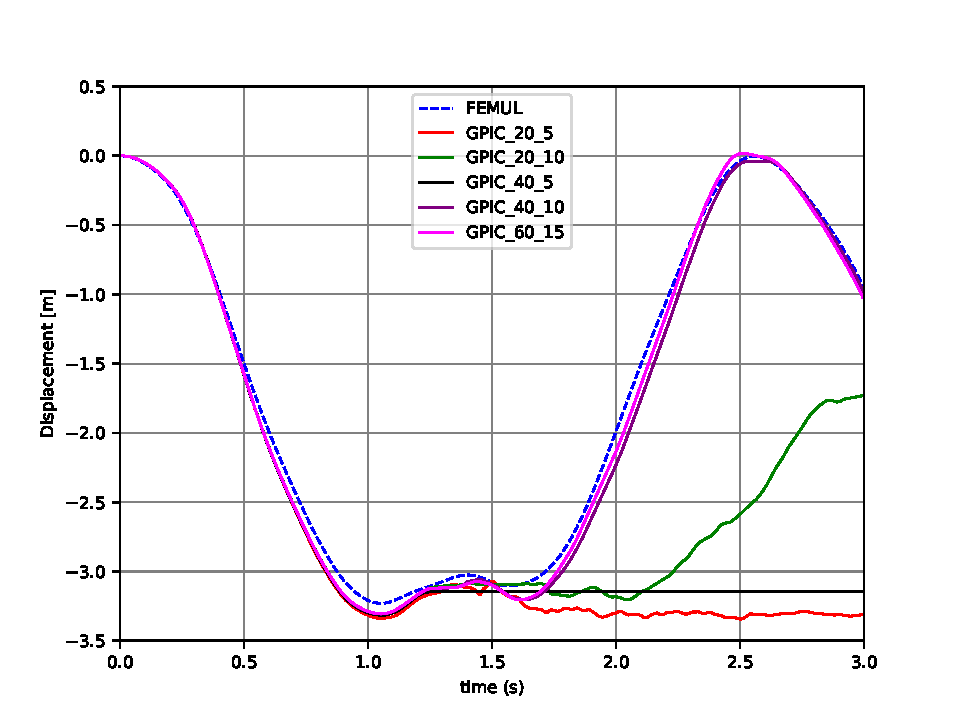
\includegraphics[width=1.0\textwidth]{vibratingbeamGPIC.pdf}
	\caption{Vibration of a compliant beam: FEM versus GPIC-mesh sensitive test}
	\label{Fig1}
\end{figure}

Important note (29/06/2023) if both coarse meshes are used for FE and background, the results seem good. So now, we have to got the analytical explanation for this results. 

The GPIC method has two meshes: background and solid FE ones. This investigation focuses on the ratio between two rectangular mesh.

%% The Appendices part is started with the command \appendix;
%% appendix sections are then done as normal sections
%% \appendix

%% \section{}
%% \label{}

%% For citations use: 
%%       \citet{<label>} ==> Jones et al. [21]
%%       \citep{<label>} ==> [21]
%%
%%%%%%%%%%%%%%%%%%%%%%%%%%%%%%
\section{Dynamic relaxation methods for form-finding problems of tensegrity structures}
\label{sec:2}

%============================================================================================================
\subsection{Equilibrium equations}\label{subsec:2:1}

%============================================================================================================
\subsection{Viscous damping approach of Dynamic relaxation method} \label{subsec:2:2}
%------------------------------------------------------------------------------------------------------------
\subsubsection{Papadrakakis method}
%------------------------------------------------------------------------------------------------------------
\subsubsection{Underwood method}
%------------------------------------------------------------------------------------------------------------
\subsubsection{Rezaiee-Pajand method}
%------------------------------------------------------------------------------------------------------------
\subsubsection{Viscous damping algorithm} 

%============================================================================================================
\subsection{Kinetic damping approach of Dynamic relaxation method} \label{subsec:2:3}

%------------------------------------------------------------------------------------------------------------
\subsubsection{Topping method}

%------------------------------------------------------------------------------------------------------------
\subsubsection{Alamatian method}

%------------------------------------------------------------------------------------------------------------
\subsubsection{Kinetic damping algorithm}

%%%%%%%%%%%%%%%%%%%%%%%%%%%%%
\section{A combination between Genetic algorithm and DR methods for form-finding problems of tensegrity structures}
\label{sec:3}

%%%%%%%%%%%%%%%%%%%%%%%%%%%%%%%%%%%%%%%%%%%%%%%%%%%%%%%%%%%%%%%%%%%
\section{Analytical Samples} \label{subsec:4} 
%-----------------------------

%%%%%%%%%%%%%%%%%%%%%%%%%%%%%%%%%%%%%%%%%%%%%%%%%%%%%%%%%%%%%%%%%%%
\section{Conclusions}

%%
\bibliographystyle{elsarticle-num-names} 
%%\bibliography{C:¥Users¥bqhie¥Dropbox¥BQH Work¥Research Project¥Project of MPM¥JabrefLibrary¥mpm}
%%\bibliography{./mpm}
%%\bibliography{./mpm-only}
\bibliography{mpm}
%% else use the following coding to input the bibitems directly in the
%% TeX file.

%\begin{thebibliography}{00}

%% \bibitem[Author(year)]{label}
%% Text of bibliographic item

%\bibitem[ ()]{}

%\end{thebibliography}
\end{document}

\endinput
%%
%% End of file `elsarticle-template-num-names.tex'.
